%%%%%%%%%%%%%%%%%%%%%%%%%%%%%%%%%%%%%%%%%%%%%%%%%%%%%%%%%%%%%%%%%%%%%%%%%%%%%%%%
% Tutorial slides on Python.
%
% Author: Prabhu Ramachandran <prabhu at aero.iitb.ac.in>
% Copyright (c) 2005-2009, Prabhu Ramachandran
%%%%%%%%%%%%%%%%%%%%%%%%%%%%%%%%%%%%%%%%%%%%%%%%%%%%%%%%%%%%%%%%%%%%%%%%%%%%%%%%

\documentclass[compress,14pt]{beamer}
% \documentclass[handout]{beamer}
% \usepackage{pgfpages}
% \pgfpagesuselayout{4 on 1}[a4paper,border, shrink=5mm,landscape]
\usepackage{tikz}
\newcommand{\hyperlinkmovie}{}
%\usepackage{movie15}

%%%%%%%%%%%%%%%%%%%%%%%%%%%%%%%%%%%%%%%%%%%%%%%%%%%%%%%%%%%%%%%%%%%%%%%%%%%%%%
% Note that in presentation mode 
% \paperwidth  364.19536pt
% \paperheight 273.14662pt
% h/w = 0.888


\mode<presentation>
{
  \usetheme{Warsaw}
  %\usetheme{Boadilla}
  %\usetheme{default}
  \useoutertheme{infolines}
  \setbeamercovered{transparent}
}

% To remove navigation symbols
\setbeamertemplate{navigation symbols}{}

\usepackage{amsmath}
\usepackage[english]{babel}
\usepackage[latin1]{inputenc}
\usepackage{times}
\usepackage[T1]{fontenc}

% Taken from Fernando's slides.
\usepackage{ae,aecompl}
\usepackage{mathpazo,courier,euler}
\usepackage[scaled=.95]{helvet}
\usepackage{pgf}

\definecolor{darkgreen}{rgb}{0,0.5,0}

\usepackage{listings}
\lstset{language=Python,
    basicstyle=\ttfamily\bfseries,
    commentstyle=\color{red}\itshape,
  stringstyle=\color{darkgreen},
  showstringspaces=false,
  keywordstyle=\color{blue}\bfseries}

%%%%%%%%%%%%%%%%%%%%%%%%%%%%%%%%%%%%%%%%%%%%%%%%%%%%%%%%%%%%%%%%%%%%%%
% My Macros
\setbeamercolor{postit}{bg=yellow,fg=black}
\setbeamercolor{emphbar}{bg=blue!20, fg=black}
\newcommand{\emphbar}[1]
{\begin{beamercolorbox}[rounded=true]{emphbar} 
      {#1}
 \end{beamercolorbox}
}
%{\centerline{\fcolorbox{gray!50} {blue!10}{
%\begin{minipage}{0.9\linewidth}
%    {#1} 
%\end{minipage}
%    }}}

\newcommand{\myemph}[1]{\structure{\emph{#1}}}
\newcommand{\PythonCode}[1]{\lstinline{#1}}

\newcommand{\tvtk}{\texttt{tvtk}}
\newcommand{\mlab}{\texttt{mlab}}

\newcounter{time}
\setcounter{time}{0}
\newcommand{\inctime}[1]{\addtocounter{time}{#1}{\vspace*{0.1in}\tiny \thetime\ m}}

\newcommand\BackgroundPicture[1]{%
  \setbeamertemplate{background}{%
      \parbox[c][\paperheight]{\paperwidth}{%
      \vfill \hfill
 \hfill \vfill
}}}

%%%%%%%%%%%%%%%%%%%%%%%%%%%%%%%%%%%%%%%%%%%%%%%%%%%%%%%%%%%%%%%%%%%%%%
% Configuring the theme
%\setbeamercolor{normal text}{fg=white}
%\setbeamercolor{background canvas}{bg=black}



%%%%%%%%%%%%%%%%%%%%%%%%%%%%%%%%%%%%%%%%%%%%%%%%%%%%%%%%%%%%%%%%%%%%%%
% Title page
\title[3D Plotting]{3D data Visualization}

\author[FOSSEE] {FOSSEE}

\institute[IIT Bombay] {Department of Aerospace Engineering\\IIT Bombay}
\date[] {12 January, 2010\\Day 2, Session 5}

%%%%%%%%%%%%%%%%%%%%%%%%%%%%%%%%%%%%%%%%%%%%%%%%%%%%%%%%%%%%%%%%%%%%%%

%\pgfdeclareimage[height=0.75cm]{iitblogo}{iitblogo}
%\logo{\pgfuseimage{iitblogo}}

\AtBeginSection[]
{
  \begin{frame}<beamer>
    \frametitle{Outline}      
    \tableofcontents[currentsection,currentsubsection]
  \end{frame}
}

%% Delete this, if you do not want the table of contents to pop up at
%% the beginning of each subsection:
\AtBeginSubsection[]
{
  \begin{frame}<beamer>
    \frametitle{Outline}
    \tableofcontents[currentsection,currentsubsection]
  \end{frame}
}

\AtBeginSection[]
{
  \begin{frame}<beamer>
    \frametitle{Outline}
    \tableofcontents[currentsection,currentsubsection]
  \end{frame}
}
%%%%%%%%%%%%%%%%%%%%%%%%%%%%%%%%%%%%%%%%%%%%%%%%%%%%%%%%%%%%%%%%%%%%%%
% DOCUMENT STARTS
\begin{document}

\begin{frame}
  \maketitle
\end{frame}

\begin{frame}
  \frametitle{Outline}
  \tableofcontents
  % You might wish to add the option [pausesections]
\end{frame}

\section{3D Data Visualization}

\begin{frame}
    \frametitle{What is visualization?}
    \Large
    \begin{center}
    Visual representation of data
    \end{center}
\end{frame}


%% \begin{frame}
%%     \frametitle{Is this new?}    
%%     \begin{center}
%%     We have moved from:
%%     \end{center}
%%     \begin{columns}
%%     \column{}
%%     \hspace*{-1in}    
%%     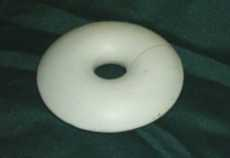
\includegraphics[width=1.75in,height=1.75in, interpolate=true]{data/3832}      
%%     \column{}\hspace*{-0.25in}
%%     To
%%     \column{}
%%     \hspace*{-1in}
%%     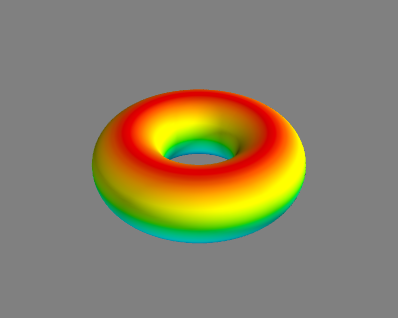
\includegraphics[width=1.75in, height=1.75in, interpolate=true]{data/torus}  
%%     \end{columns}
%% \end{frame}

\begin{frame}
    \frametitle{3D visualization}
    \Large
    \begin{center}
        Harder but important
    \end{center}
\end{frame}

\begin{frame}
    \frametitle{Is this Graphics?}
    \Large
    \begin{center}
        Visualization is about data!
    \end{center}
\end{frame}

\begin{frame}
    \frametitle{Examples: trajectory in space}
    \Large
    \begin{center}
        \pgfimage[width=2.5in]{MEDIA/m2/mlab/plot3d_ex}
    \end{center}
\end{frame}

\begin{frame}
    \frametitle{Examples: Fire in a room}
    \Large
    \begin{center}
        Demo of data
    \end{center}
\inctime{10}
\end{frame}

\section{Tools available}

\subsection{mlab}

\begin{frame}
    {Overview}
    \Large
    \begin{itemize}
        \item Simple
        \item Convenient
        \item Full-featured
    \end{itemize}
\end{frame}

\begin{frame}[fragile]

    \frametitle{Getting started}
    \myemph{\Large Vanilla:}
    \begin{lstlisting}[language=bash]
        $ ipython -wthread
    \end{lstlisting}
    \myemph{\Large with Pylab:}
    \begin{lstlisting}[language=bash]
        $ ipython -pylab -wthread
    \end{lstlisting}
\end{frame}

\begin{frame}[fragile]
    \frametitle{Using mlab}

    \begin{lstlisting}
In []:from enthought.mayavi import mlab
    \end{lstlisting}

    \vspace*{0.5in}

    \myemph{\Large Try these}

    \vspace*{0.25in}

    \begin{lstlisting}
In []: mlab.test_<TAB>
In []: mlab.test_contour3d()
In []: mlab.test_contour3d??
    \end{lstlisting}
\end{frame}

\begin{frame}
    {Exploring the view}
    \begin{columns}
        \column{0.6\textwidth}
    \pgfimage[width=3in]{MEDIA/m2/contour3d}
        \column{0.4\textwidth}
        \begin{itemize}
            \item Mouse
            \item Keyboard
            \item Toolbar
            \item Mayavi icon\pgfimage[width=0.2in]{MEDIA/m2/m2_icon}
        \end{itemize}
    \end{columns}
\end{frame}

\begin{frame}[fragile]
    \frametitle{\mlab\ plotting functions}
    \begin{columns}
        \column{0.25\textwidth}
        \myemph{\Large 0D data}
        \column{0.5\textwidth}
    \pgfimage[width=2in]{MEDIA/m2/mlab/points3d_ex}
    \end{columns}

    \begin{lstlisting}
In []: t = linspace(0, 2*pi, 50)
In []: u = cos(t) * pi
In []: x, y, z = sin(u), cos(u), sin(t)
    \end{lstlisting}
    \emphbar{\PythonCode{In []: mlab.points3d(x, y, z)}}
\end{frame}

\begin{frame}
  \begin{columns}
        \column{0.25\textwidth}
        \myemph{\Large 1D data}
        \column{0.5\textwidth}
        \pgfimage[width=2.5in]{MEDIA/m2/mlab/plot3d_ex}
  \end{columns}
  \emphbar{\PythonCode{In []: mlab.plot3d(x, y, z, t)}}

    Plots lines between the points
    
\end{frame}

\begin{frame}[fragile]
    \begin{columns}
        \column{0.25\textwidth}
        \myemph{\Large 2D data}
        \column{0.5\textwidth}
        \pgfimage[width=2in]{MEDIA/m2/mlab/surf_ex}
    \end{columns}            
    \begin{lstlisting}
In []: x, y = mgrid[-3:3:100j,-3:3:100j]
In []: z = sin(x*x + y*y)
    \end{lstlisting}

    \emphbar{\PythonCode{In []: mlab.surf(x, y, z)}}

    \alert{Assumes the points are rectilinear}

\end{frame}

\begin{frame}[fragile]
  \frametitle{mgrid}
  \begin{lstlisting}
In []: mgrid[0:3,0:3]
Out[]: 
array([[[0, 0, 0],
        [1, 1, 1],
        [2, 2, 2]],

       [[0, 1, 2],
        [0, 1, 2],
        [0, 1, 2]]])

In []: mgrid[-1:1:5j]
Out[]: array([-1., -0.5,  0.,  0.5,  1.])
\end{lstlisting}
\end{frame}

\begin{frame}[fragile]
  \frametitle{Example}
  \begin{lstlisting}
In []: x, y = mgrid[-1:1:5j, -1:1:5j]
In []: z = x*x + y*y

In []: z
Out[]: 
array([[ 2.  , 1.25, 1.  , 1.25, 2.  ],
       [ 1.25, 0.5 , 0.25, 0.5 , 1.25],
       [ 1.  , 0.25, 0.  , 0.25, 1.  ],
       [ 1.25, 0.5 , 0.25, 0.5 , 1.25],
       [ 2.  , 1.25, 1.  , 1.25, 2.  ]])
\end{lstlisting}
\end{frame}

\begin{frame}[fragile]
    \myemph{\Large 2D data: \texttt{mlab.mesh}}
    \vspace*{0.25in}

    \emphbar{\PythonCode{In []: mlab.mesh(x, y, z)}}

    \alert{Points needn't be regular}

    \vspace*{0.25in}
\begin{lstlisting}
In []: phi, theta = mgrid[0:pi:20j, 
...                         0:2*pi:20j]
In []: x = sin(phi)*cos(theta)
In []: y = sin(phi)*sin(theta)
In []: z = cos(phi)
In []: mlab.mesh(x, y, z, 
...           representation=
...           'wireframe')
\end{lstlisting}

\end{frame}

\begin{frame}[fragile]

  \begin{columns}
        \column{0.25\textwidth}
        \myemph{\Large 3D data}
        \column{0.5\textwidth}
        \pgfimage[width=1.5in]{MEDIA/m2/mlab/contour3d}\\        
    \end{columns}
\begin{lstlisting}
In []: x, y, z = mgrid[-5:5:64j, 
...                -5:5:64j, 
...                -5:5:64j]
In []: mlab.contour3d(x*x*0.5 + y*y + 
                   z*z*2)
\end{lstlisting}
\end{frame}

\begin{frame}[fragile]

    \myemph{\Large 3D vector data: \PythonCode{mlab.quiver3d}}
    \vspace*{0.25in}

    \pgfimage[width=2in]{MEDIA/m2/mlab/quiver3d_ex}\\
    
\begin{lstlisting}
In []: mlab.test_quiver3d()
\end{lstlisting}

\emphbar{\PythonCode{obj = mlab.quiver3d(x, y, z, u, v, w)}}
\inctime{20}
\end{frame}


\subsection{Mayavi2}

\begin{frame}
  \frametitle{Introduction to Mayavi}
  \begin{itemize}
  \item Most scientists not interested in details of visualization
  \item Visualization of data files with a nice UI
  \item Interactive visualization of data (think Matlab)
  \item Embedding visualizations in applications
  \item Customization
  \end{itemize}
  \pause
  \begin{block}{The Goal}
      Provide a \alert{flexible} library/app for all of these needs!
  \end{block}
\end{frame}

\begin{frame}
    {Overview of features}
      \vspace*{-0.3in}
  \begin{center}    
    \hspace*{-0.2in}\pgfimage[width=5in]{MEDIA/m2/m2_app3_3}
  \end{center}    
\end{frame}


\begin{frame}
    \frametitle{Mayavi in applications}
      \vspace*{-0.3in}
  \begin{center}    
    \hspace*{-0.2in}\pgfimage[width=4.5in]{MEDIA/m2/m2_envisage}
  \end{center}
\end{frame}

\begin{frame}
    \frametitle{Live in your dialogs}
      \vspace*{0.1in}
  \begin{center}    
    \hspace*{-0.2in}\pgfimage[width=2.5in]{MEDIA/m2/mlab_tui}
  \end{center}
\end{frame}

\begin{frame}
    {Exploring the documentation}
    \begin{center}
    \pgfimage[width=4in]{MEDIA/m2/m2_ug_doc}
    \end{center}
\end{frame}


\begin{frame}
  \frametitle{Summary}
      \begin{itemize}
          \item \url{http://code.enthought.com/projects/mayavi}
          \item Uses VTK (\url{www.vtk.org})
          \item BSD license
          \item Linux, win32 and Mac OS X
          \item Highly scriptable
          \item Embed in Traits UIs (wxPython and PyQt4)
          \item Envisage Plugins
          \item Debian/Ubuntu/Fedora
          \item \alert{Pythonic}
      \end{itemize}
    
      \inctime{10}

\end{frame}

\begin{frame}
    {Getting hands dirty!}

        \begin{block}{Motivational problem}
        Atmospheric data of temperature over the surface of the earth.
        Let temperature ($T$) vary linearly with height ($z$):
        \begin{center}            
        $T = 288.15 - 6.5z$
        \end{center}
        \end{block}
\end{frame}

\begin{frame}[fragile]
    \frametitle{Simple solution}

    \begin{lstlisting}
lat = linspace(-89, 89, 37)
lon = linspace(0, 360, 37)
z = linspace(0, 100, 11)
    \end{lstlisting}
\pause
    \begin{lstlisting}
x, y, z = mgrid[0:360:37j,-89:89:37j,
                0:100:11j]
t = 288.15 - 6.5*z
mlab.contour3d(x, y, z, t)
mlab.outline()
mlab.colorbar()
    \end{lstlisting}
\end{frame}

\begin{frame}[fragile]
    \frametitle{Exercise: Lorenz equation}
    \begin{columns}
        \column{0.25\textwidth}
        \begin{eqnarray*}
        \frac{d x}{dt} &=& s (y-x)\\
        \frac{d y}{d t} &=& rx -y -xz\\
        \frac{d z}{d t} &=& xy - bz\\
        \end{eqnarray*}
        \column{0.25\textwidth}
        Let $s=10,$
        $r=28,$ 
        $b=8./3.$
    \end{columns}
    \structure{\Large Region of interest}
  \begin{lstlisting}
x, y, z = mgrid[-50:50:20j,-50:50:20j,
                -10:60:20j]
  \end{lstlisting}
\inctime{20}

\end{frame}
\begin{frame}[fragile]
    \frametitle{Solution}
  \begin{lstlisting}
def lorenz(x,y,z,s=10.,r=28.,b=8./3.):
    u = s*(y-x)
    v = r*x-y-x*z
    w = x*y-b*z
    return u,v,w
x,y,z = mgrid [-50:50:20j,-50:50:20j,
                    -10:60:20j ]
u,v,w = lorenz( x , y , z )
# Your plot here
#
mlab.show()

  \end{lstlisting}
\end{frame}

\begin{frame}
  \frametitle{We have covered:}
  \begin{itemize}
  \item Need of visualization.
  \item Using mlab to create 3 D plots.
  \item Mayavi Toolkit.
  \end{itemize}
\end{frame}

\end{document}

